\chapter{TẬP DỮ LIỆU}

\section{Khảo sát dữ liệu}
Như đã đề cập ở Chương \ref{chapter:introduction}, không có nhiều tập dữ liệu được gắn nhãn về gan và mạch máu được công khai. Sau đây là một số tập dữ liệu phổ biến sẽ được dùng để nghiên cứu.
Mô hình phân đoạn gan sẽ sử dụng cả 3 tập dữ liệu được đề cập. Mô hình phân đoạn mạch máu sẽ chỉ dùng tập dữ liệu 3DIRCAD (vì hiện tại chỉ có tập dữ liệu này được gán nhãn mạch máu được công bố).

\subsection{Liver Tumor Segmentation Challenge 2017}
\textbf{Liver Tumor Segmentation Challenge (LITS2017)}\cite{lits}: là tập dữ liệu được sử dụng trong cuộc thi phân đoạn gan và khối u gan do ISBI và MICCAI hợp tác tổ chức vào năm 2017. Tập dữ liệu bao gồm 131 ảnh CT có gắn nhãn dùng để huấn luyện và 70 ảnh CT chưa có nhãn dùng để đánh giá. Bộ dữ liệu được thu thập bởi các máy quét và giao thức khác nhau từ sáu vị trí lâm sàng khác nhau, với độ phân giải trong mặt phẳng thay đổi lớn từ 0,55 mm đến 1,0 mm và khoảng cách lát từ 0,45 mm đến 6,0 mm.\par

 Dữ liệu gồm các file \textit{volume} được đánh số từ 0 đến 130 là ảnh CT, cùng với đó là các file \textit{segmentation} là nhãn tương ứng cũng được đánh số từ 0 đến 130. Tất cả các file đều ở định dạnh 'nii'. Trong đó có 118 ảnh chứa khối u trên tổng số 131 bộ ảnh CT.

\begin{figure}[H]
    \centering
    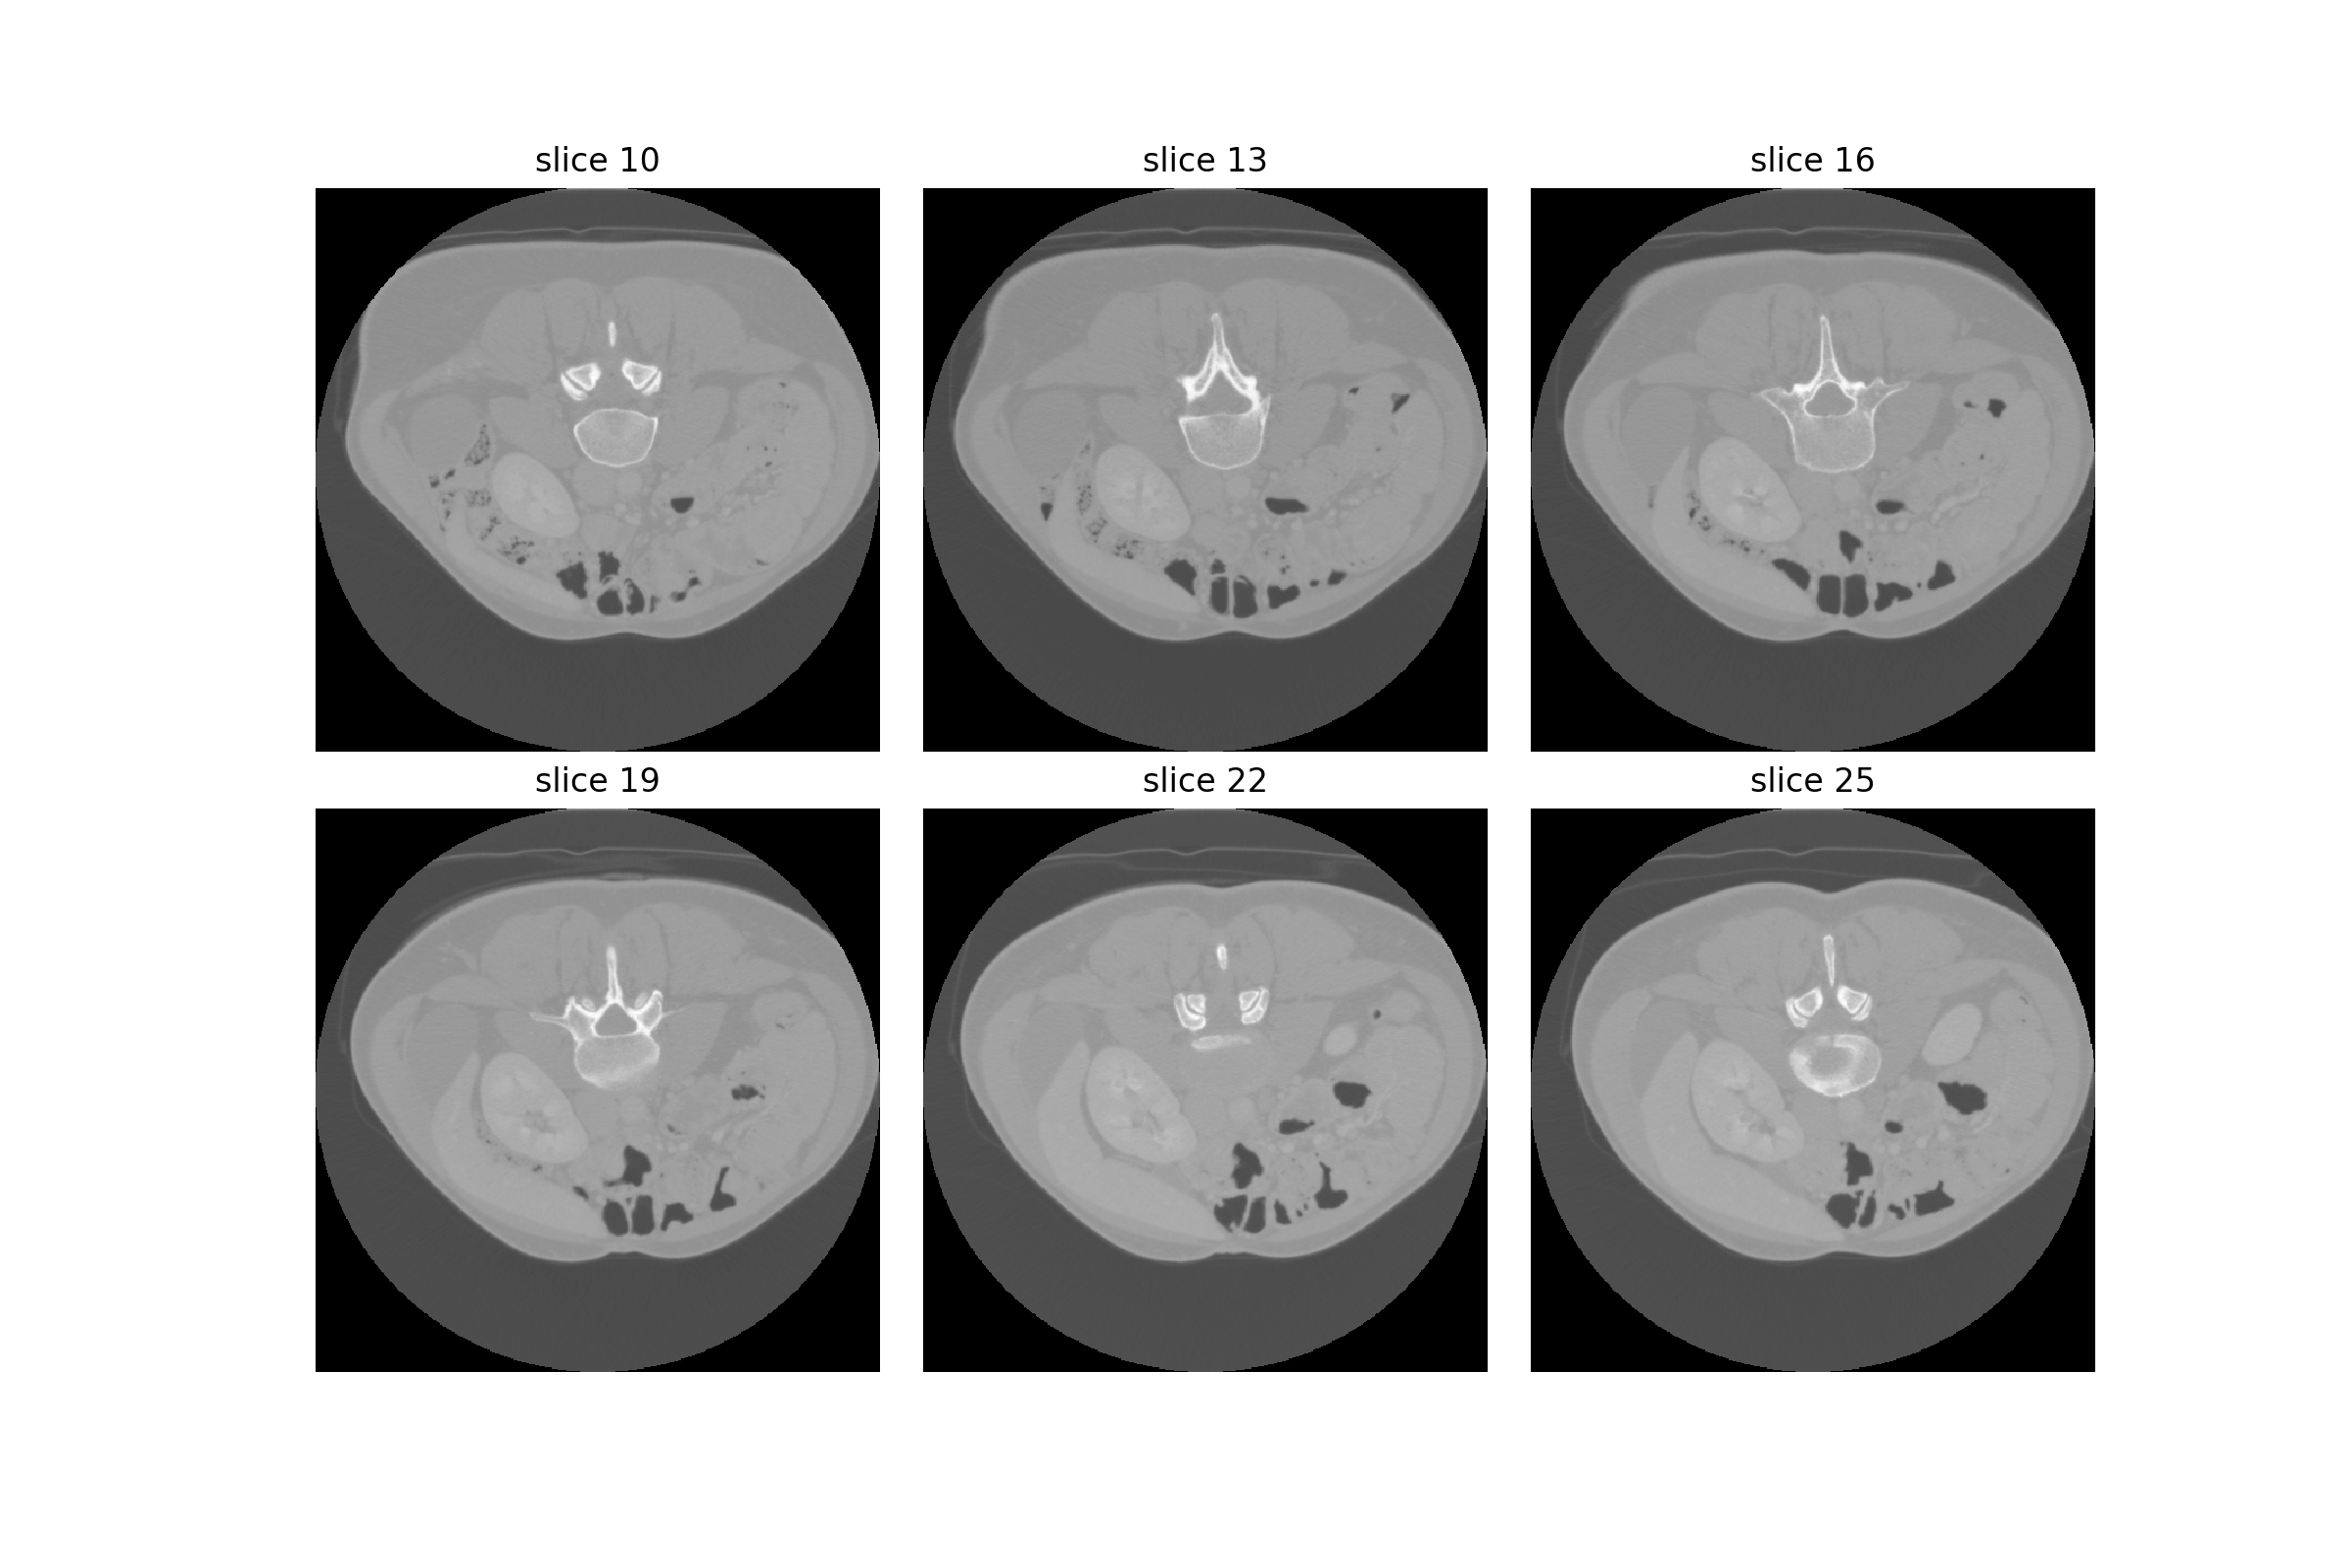
\includegraphics[width=10cm]{images/experience/volume-35-6slice.png}
    \caption{Một vài lát cắt trong ảnh volume-35 lấy từ tập dữ liệu LITS2017.}
\end{figure}
Tất cả các lát cắt đều có kích thước $512\times 512$ nhưng số lượng mỗi lát cắt trong mỗi ảnh CT là khác nhau. Cụ thể tính trên 130 ảnh huấn luyện, số lát cắt nhỏ nhất là 74, lớn nhất là 987 và trung bình là 448.\par
Như đã đề cập, dữ liệu bị mất cân bằng nghiêm trọng giữa phần nền và phần gan. 

\begin{figure}[H]
  \centering
  \subfloat[Tỉ lệ thể tích của gan đối với nền]{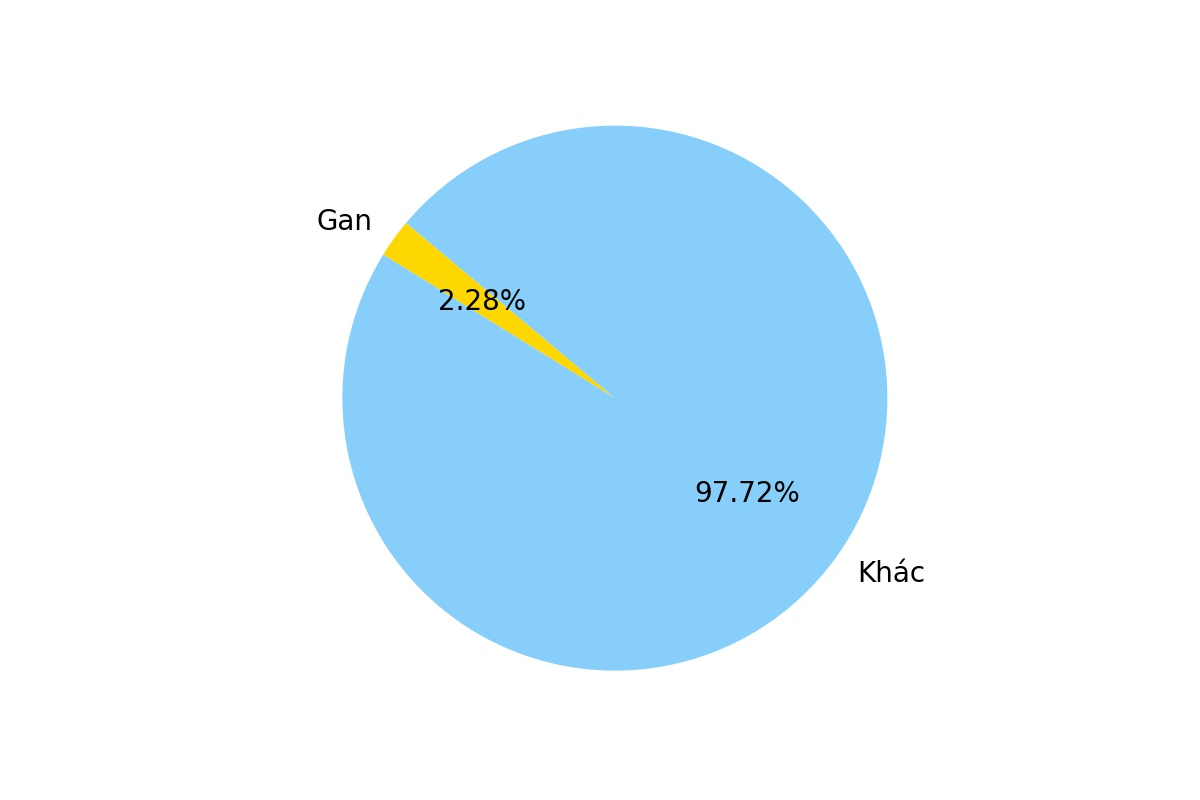
\includegraphics[width=0.45\textwidth]{images/experience/liver_background.jpg}\label{fig:f1}}
  \hfill
  \subfloat[Tỉ lệ thể tích của khối u so với gan]{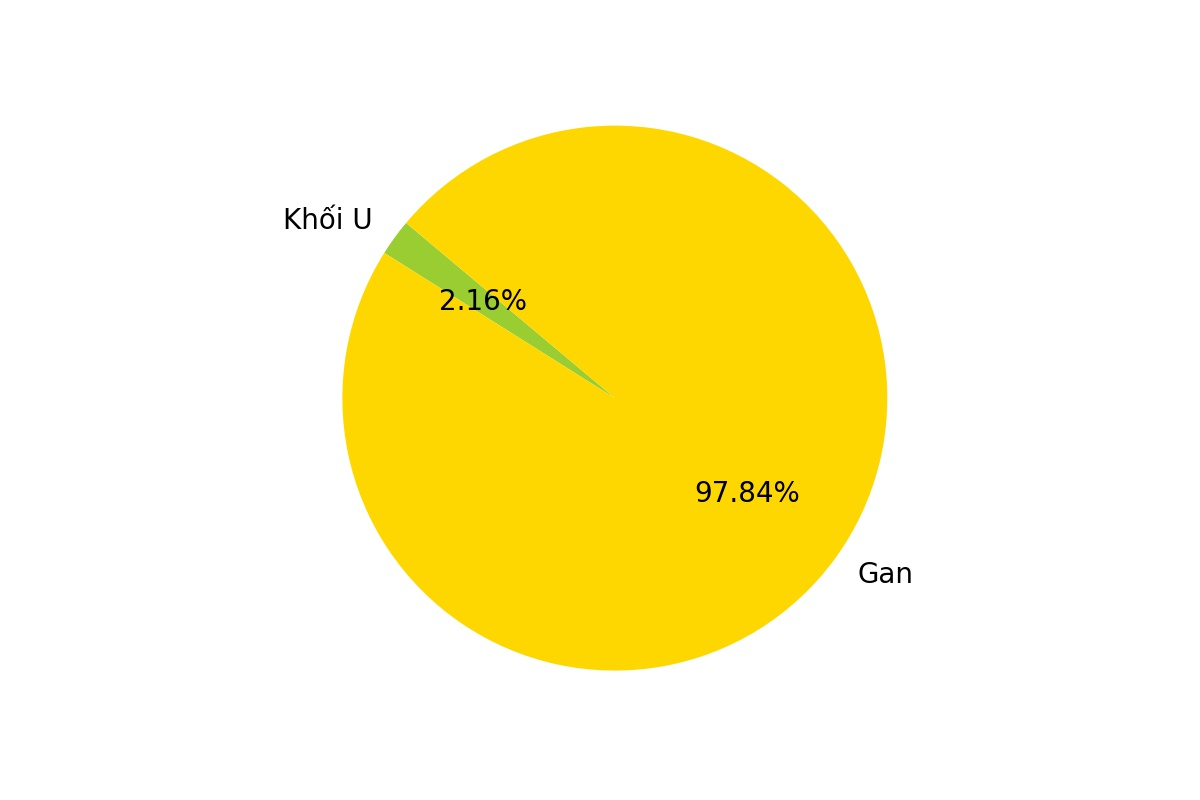
\includegraphics[width=0.45\textwidth]{images/experience/tumor_liver.jpg}\label{fig:f2}}
  \caption{Tỉ lệ thể tích của gan, khối u và nền trên tập huấn luyện LITS2017.}
\end{figure}

Qua biểu đồ, ta thấy rằng thể tích gan chỉ chiếm 2.28\% trong khi phần nền chiếm tới 97.72\%, u chỉ chiếm hơn 2\% trên tổng thể tích của gan, đặc biệt khi xem xét đến tỉ lệ thể tích của khối u so với nền, đây thực sự là một thách thức lớn.\par

\subsection{Segmentation of the Liver 2007}
\textbf{Segmentation of the Liver 2007 (SLIVER07)} \cite{sliver07}: Đây là tập dữ liệu được sử dụng trong
một cuộc thi thuộc khuôn khổ hội nghị MICCAI 2007 dành cho các hệ thống \textit{phân đoạn
lá gan} tự động và bán tự động. Trong đó gồm 20 ảnh CT có gắn nhãn phục vụ mục đích huấn luyện và 10 ảnh CT không nhãn để chấm điểm online. Số mặt cắt trong tập ảnh nằm trong khoảng từ 64 đến 388
ảnh 2-chiều. Khoảng cách mỗi điểm ảnh trong mỗi ảnh cắt ngang nằm trong khoảng 0.55
đến 0.8 mi-li-mét, khoảng cách hai mặt cắt liên tiếp từ 1 đến 3 mi-li-mét. Mỗi ảnh CT
đều đi kèm với các thông số trên. 

\subsection{3Dircadb}
\textbf{3D Image Reconstruction for Comparison of Algorithm Database (3Dircadb)} \cite{3dircad}: Đây là tập dữ liệu do Viện nghiên cứu chống ung thư đường tiêu hóa của trường Đại học Bệnh viện IRCAD tại Pháp cung cấp. Đây là tập dữ liệu chứa thông tin gần như đầy đủ các cơ quan trong lồng ngực gồm: phổi, gan, xương, động/tĩnh mạch, thận, khối u gan... Do đó việc huấn luyện mô hình phân đoạn mạch máu sẽ tập trung vào tập dữ liệu này. \par

3D-IRCADb có hai gói dữ liệu là 3D-IRCADb-01 và 3D-IRCADb-02. Chúng tôi chọn sử dụng gói 3D-IRCADb-01 tiến hành huấn luyện và đánh giá hệ thống phân đoạn trong luận văn này. Tập dữ liệu này cung cấp một số bộ ảnh y khoa từ các bệnh nhân được ẩn danh bao gồm 20 ảnh CT lồng ngực của 20 bệnh nhân (10 nam - 10 nữ) và các cơ quan của từng bệnh nhân được gán nhãn bằng phương pháp thủ công bởi các chuyên gia lâm sàng. \par

 3D-IRCADb-01 bao gồm các bộ ảnh CT với sự xuất hiện của khối u gan trong 75\% các trường hợp. Hệ thống mạch máu trong các bộ ảnh CT được chia thành ba phần là \textit{tĩnh mạch chủ}, \textit{tĩnh mạch cửa} và \textit{động mạch} và được phân đoạn riêng cho từng loại mạch máu. Số mặt cắt trong tập ảnh nằm trong khoảng từ 91 đến 260 ảnh 2-chiều. Các ảnh trong tập dữ liệu này có các khoảng cách giữa các điểm ảnh từ 0,56mm đến 0,81mm, khoảng cách hai mặt cắt từ 1,6mm đến 4mm. Hình \ref{3dircad_sample} là ảnh trực quan dữ liệu cho từng bệnh nhân trong gói 3D-IRCADb-01. 

\begin{figure}[H]
    \centering
    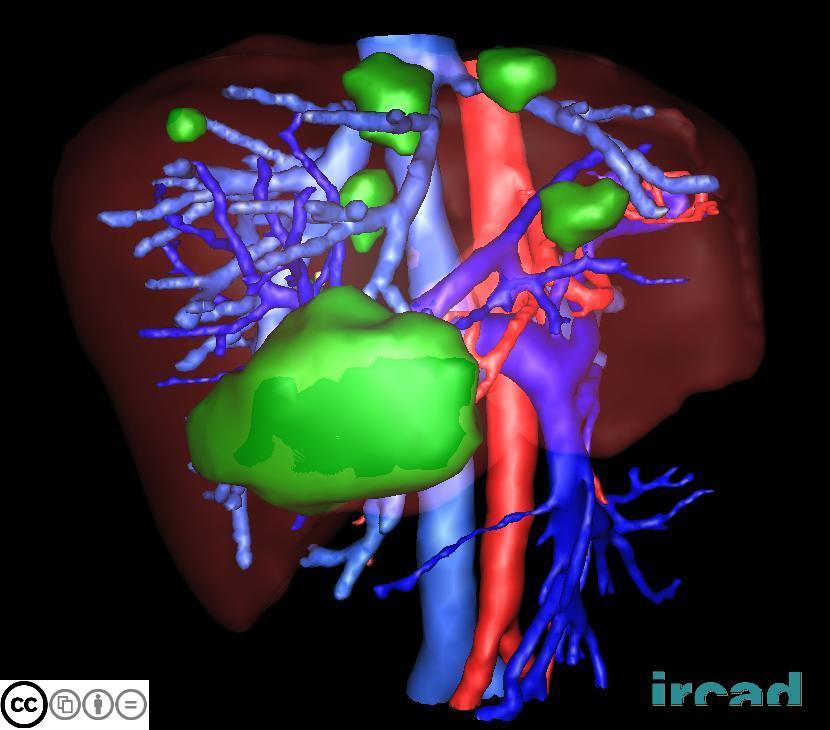
\includegraphics[width=8cm]{images/dataset/3Dircadb1.jpg}
    \caption{Ảnh trực quan các bộ phân được đánh nhãn trong tập dữ liệu \cite{3dircad}.}
    \label{3dircad_sample}
\end{figure}
\vspace{-10mm}

\section{Tiền xử lý dữ liệu}
\subsection{Chuẩn bị dữ liệu} \label{data-preparation}
Đối với các giải thuật học máy hiện nay, khâu chuẩn bị dữ liệu là vô cùng quan trọng. Cụ thể hơn học sâu là một phần của một họ các phương pháp học máy rộng hơn dựa trên đại diện học của một tập dữ liệu. Do đó nếu chúng ta sử dụng một mô hình được học trên tập dữ liệu có phân bố khác với tập kiểm tra thì kết quả dự đoán của mô hình không thể đạt được sự chính xác như ta kì vọng. Do đó ta cần phải có 1 khảo sát để xác định một phương pháp chia dữ liệu thích hợp.\par

Đầu tiên, trong tập 3DIRCAD gồm 20 bệnh nhân, chúng tôi tiến hành khảo sát mức độ phân bố giá trị Hounsfield Unit (của gan và máu tương ứng). \textit{Hình} \ref{hu_dist} được vẽ dựa trên giá trị trung bình (mean) và 2 lần giá trị độ lệch chuẩn (std) thể hiện 95\% giá trị HU của mạch máu (gan) phân phối trong khoảng giá trị đó. Dựa vào bệnh nhân số 8 và bệnh nhân số 9 ta có thể thấy được sự khác biệt trong phân bố giá trị HU ở cả gan và mạch máu (ở gan, bệnh nhân 8 phân bố quanh giá trị 160 trong khi đó bệnh nhân số 9 phân bố quanh giá trị 80 
đối với gan).

\begin{figure}[H]
	\begin{center}
		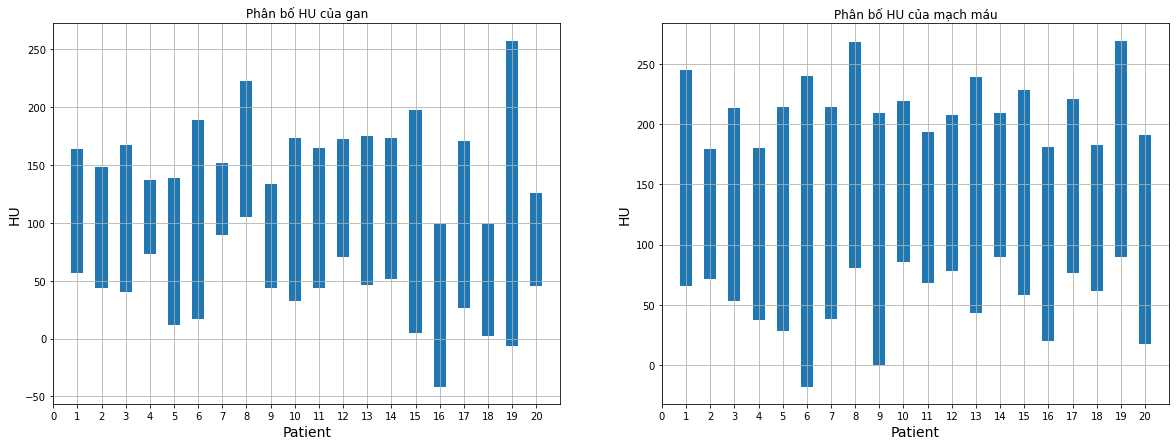
\includegraphics[width=13cm]{images/experiments/hu_dist.png}
		\caption{Phân bố giá trị HU từng bệnh nhân.}
		\label{hu_dist}
	\end{center}
	\begin{center}
		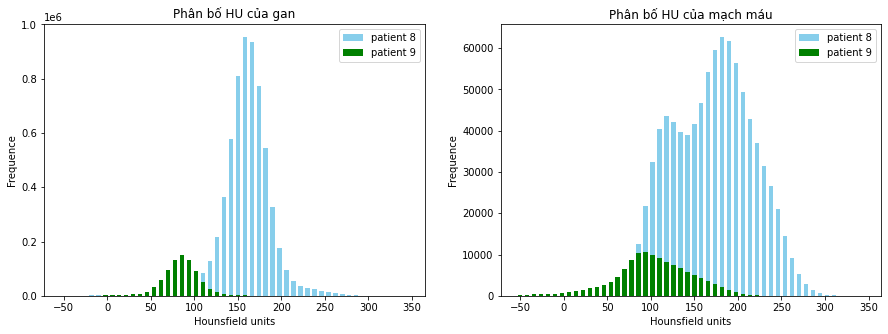
\includegraphics[width=13cm]{images/experiments/compare_2patient.png}
		\caption{So sánh phân bố HU của 2 bệnh nhân số 8 và số 9.}
		\label{hu_compare}
	\end{center}
\end{figure}
\vspace{-0.25cm}
Do đó, chúng tôi tiến hành chia tập dữ liệu thành 3 tập dữ liệu bao gồm: tập huấn luyện, tập kiểm thử, tập kiểm tra dựa trên phân phối giá trị trung bình HU của từng bệnh nhân.

\begin{table}[H]
    \centering
    \begin{tabular}{|c|l|l|l|l|c|}
    \hline
    \multicolumn{1}{|c|}{\multirow{2}{*}{\textbf{STT}}} & \multicolumn{1}{c|}{\multirow{2}{*}{\textbf{Tập}}} & \multicolumn{3}{c|}{\textbf{Phân phối giá trị trung bình HU}}       & \multirow{2}{*}{\textbf{Tổng}} \\ \cline{3-5}
    \multicolumn{1}{|c|}{}                     & \multicolumn{1}{c|}{}                     & \textless{}125 & {[}125 , 150{]}        & \textgreater 150 &                       \\ \hline
    0 & Huấn luyện   & 5, 16, 9, 18, 20  & 2, 3, 7, 12, 13, 14, 15 & 8, 10    & 14                    \\ \hline
    1 & Kiểm thử     & 4             & 17                     & 19          & 3                     \\ \hline
    2 & Kiểm tra     & 6             & 11                     & 1           & 3                     \\ \hline
    
    \end{tabular}
    \caption{Bảng phân chia các bệnh nhân thành các tập dữ liệu cho mạch máu.}
    \label{tab:training-set-vessel}
    \begin{tabular}{|c|l|l|l|l|c|}
    \hline
    \multicolumn{1}{|c|}{\multirow{2}{*}{\textbf{STT}}} & \multicolumn{1}{c|}{\multirow{2}{*}{\textbf{Tập}}} & \multicolumn{3}{c|}{\textbf{Phân phối giá trị trung bình HU}}       & \multirow{2}{*}{\textbf{Tổng}} \\ \cline{3-5}
    \multicolumn{1}{|c|}{}                     & \multicolumn{1}{c|}{}                     & \textless{}100 & {[}100 , 110{]}        & \textgreater 110 &                       \\ \hline
    0                                          & Huấn luyện                                & 2, 5, 9, 16, 17  & 1, 3, 10, 11, 15 & 7, 8, 13, 14       & 14                    \\ \hline
    1                                          & Kiểm thử                                  & 18             & 6                     & 12               & 3                     \\ \hline
    2                                          & Kiểm tra                                  & 20              & 4                     & 19              & 3                     \\ \hline
    \end{tabular}
    \caption{Bảng phân chia các bệnh nhân thành các tập dữ liệu cho gan.}
\end{table}

\subsection{Các phương pháp xử lý dữ liệu} \label{data-process}
Trong phần này, nhóm trình bày các công việc đã thực hiện để tiền xử lý dữ liệu bao gồm: lấy mẫu dữ liệu, chuẩn hóa dữ liệu, chia dữ liệu thành các khối nhỏ, tăng cường dữ liệu, trích xuất thành phần gan.
\subsubsection{Lấy mẫu dữ liệu}
Trong quá trình khảo sát các tập dữ liệu (cụ thể 3DIRCAD), chúng tôi nhận thấy khoảng cách thực giữa các điểm ảnh trong tập dữ liệu theo các chiều có sự chênh lệch lớn (Bảng \ref{voxelsize}). Điều này gây ảnh hưởng đến quá trình huấn luyện của mô hình bởi dữ liệu không đồng nhất. Do đó để chuẩn hóa dữ liệu, chúng tôi tiến hành lấy mẫu lại ảnh bằng cách đưa khoảng cách thực ban đầu về chung một giá trị đối với tất cả các ảnh. Về phương pháp thu phóng ảnh, chúng tôi sử dụng hàm nội suy bậc ba spline (do thư viện scipy cung cấp).

\begin{table}[H]
    \centering
    \begin{tabular}{|c|c|c|c|}
    \hline
    \textbf{STT} & \textbf{Giới tính} & \textbf{Kích thước voxel (mm)} & \textbf{Kích thước ảnh (pixels)} \\ \hline
    1   & Nữ  & 0.57 - 0.57 - 1.6  & 512 - 512 - 129 \\ \hline
    2   & Nữ  & 0.78 - 0.78 - 1.6  & 512 - 512 - 172 \\ \hline
    3   & Nam & 0.62 - 0.62 - 1.25 & 512 - 512 - 200 \\ \hline
    ... &     &                    &                 \\ \hline
    20  & Nữ  & 0.81 - 0.81 - 2.0  & 512 - 512 - 225 \\ \hline
    \end{tabular}
    \caption{Thông tin ảnh của tập dữ liệu 3DIRCAD (chi tiết có thể xem tại \cite{3dircad})}
    \label{voxelsize}
\end{table}

Việc lấy mẫu lại làm thay đổi đáng kể kích thước tập dữ liệu ban đầu (h - w - d). Một số chiều dữ liệu bị kéo dãn ra, một số chiều bị thu hẹp lại.

\begin{table}[H]
    \centering
    \begin{tabular}{|c|c|c|c|}
    \hline
    \multirow{2}{*}{\textbf{STT}} & \multirow{2}{*}{\textbf{Giới tính}} & \multicolumn{2}{c|}{\textbf{Kích thước ảnh sau khi nội suy (pixels)}}  \\ \cline{3-4}
     &  & \textbf{(1.0 - 1.0 - 1.0) mm} & \textbf{(0.5 - 0.5 - 0.5) mm} \\ \hline
    1   & Nữ  & 292 - 292 - 206  & 584 - 584 - 413 \\ \hline
    2   & Nữ  & 398 - 398 - 275 & 798 - 798 - 550 \\ \hline
    3   & Nam & 316 - 316 - 250 & 634 - 634 - 500 \\ \hline
    ... &     &                 &                 \\ \hline
    20  & Nữ  & 414 - 414 - 450 & 828 - 828 - 900 \\ \hline
    \end{tabular}
    \caption{Kết quả sau khi nội suy dữ liệu}
\end{table}

\subsubsection{Lấy ngưỡng giá trị Hounsfield Unit(HU)}
Để làm tăng độ tương phản giữa gan (mạch máu) và các bộ phận khác trong ảnh CT, một phương pháp được áp dụng phổ biến là chọn ngưỡng giá trị cho ảnh. Câu hỏi đặt ra lúc này là làm thế nào để chọn ngưỡng HU cho hợp lý? Chúng ta sẽ phân tích phân bố giá trị HU để chọn những giá trị ngưỡng phù hợp. Dưới đây là biểu đồ thể hiện phân phối giá trị HU của gan trên toàn bộ tập dữ liệu 3DIRCADB-01.

\begin{figure}[H]
    \centering
    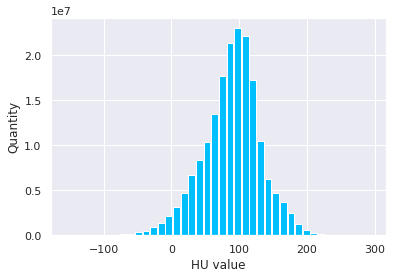
\includegraphics[width=10cm]{images/experiments/hu_dist_liver.png}
    \caption{Biểu đồ Hounsfield Units của tất cả các voxel chứa gan trên tập 3dircadb-01.}
\end{figure}
\vspace{-0.5cm}
Dựa vào biểu đồ trên, ta thấy giá trị HU của gan sẽ phân bố chủ yếu trên đoạn [-100, 250], do đó, ta sẽ chuẩn hóa dữ liệu bằng cách đưa các voxel có giá trị HU nhỏ hơn -100 về -100 và những voxel có giá trị lớn hơn 250 về 250. Nhờ vào đó ảnh trở lên tương phản hơn, đem lại thông tin rõ ràng hơn giữa các bộ phận. So sánh hình ảnh trước và sau khi thực hiện lấy ngưỡng giá trị HU:
\vspace{-0.5cm}
\begin{figure}[H]
    \centering
    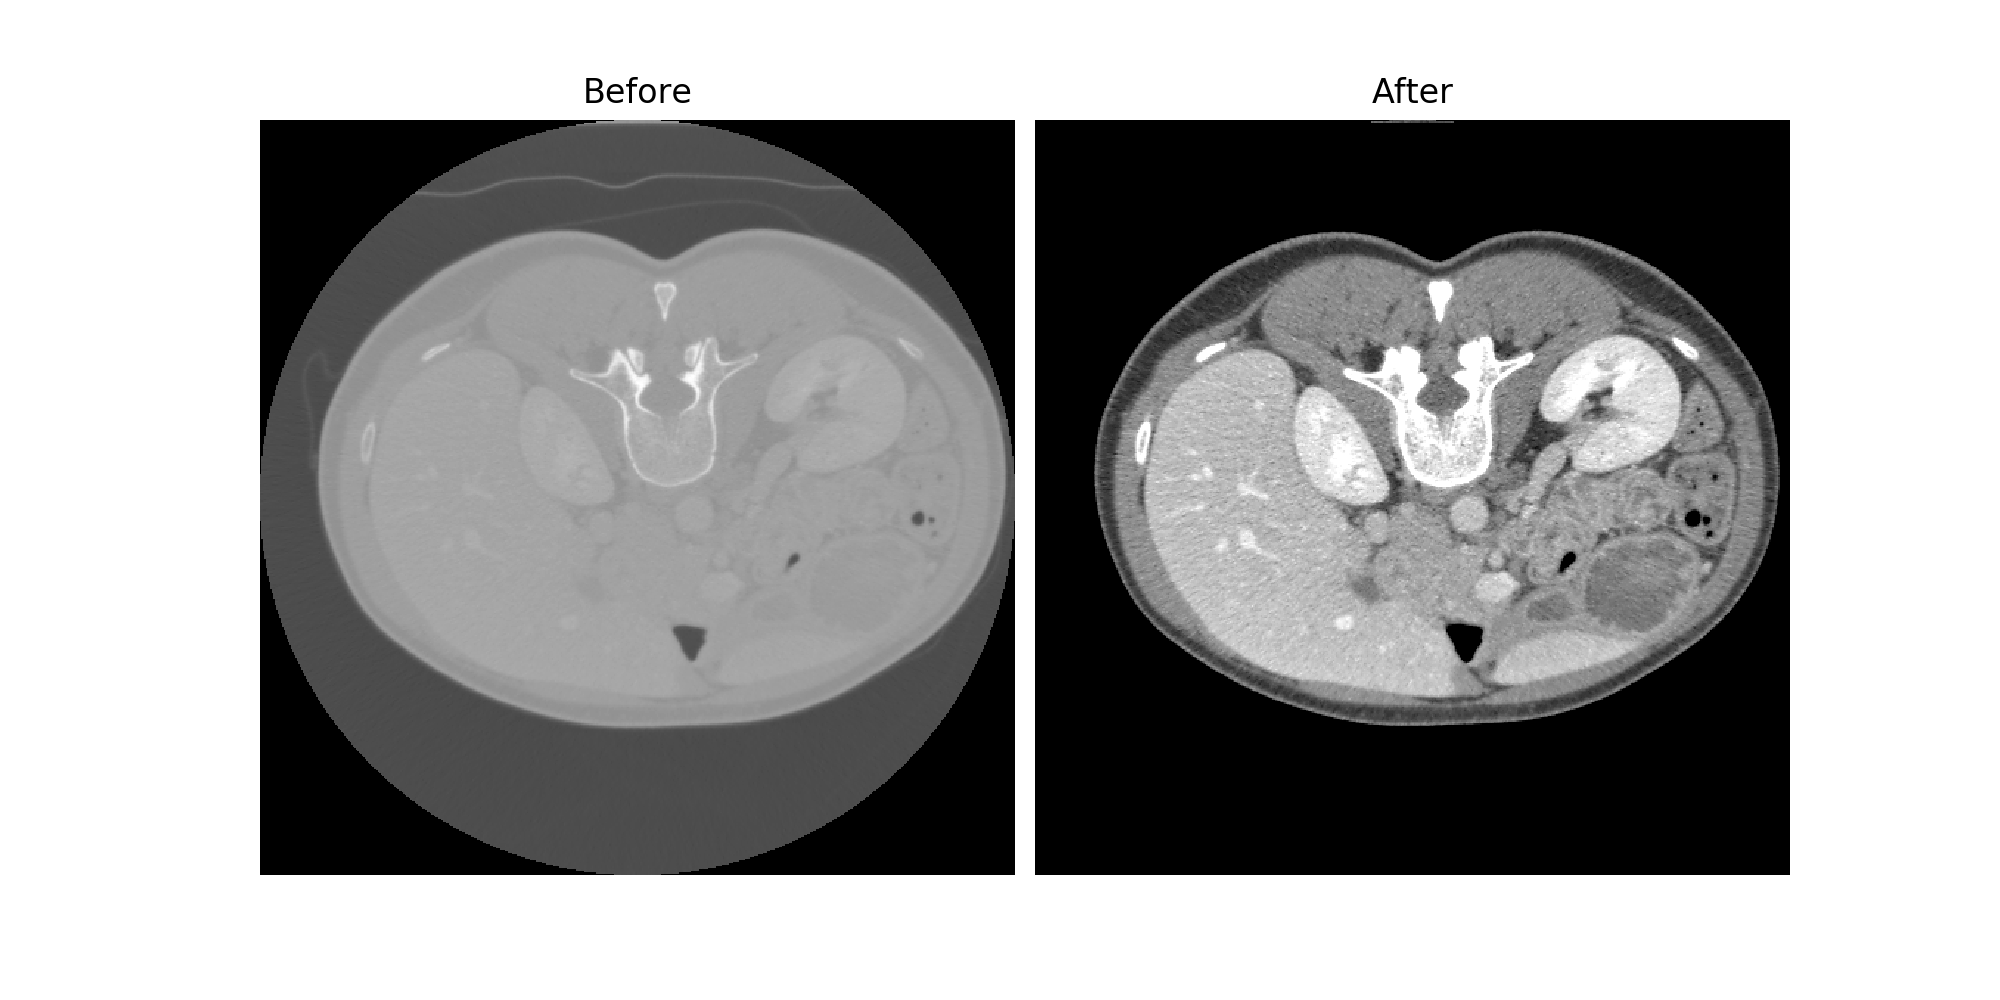
\includegraphics[width=10cm]{images/experience/HU-before-after.png}
    \caption{Kết quả trước và sau khi lấy ngưỡng giá trị HU.}
\end{figure}

\subsubsection{Chuẩn hóa dữ liệu}
Để tăng hiệu suất học tập của mô hình, sự phân bố giá trị của ảnh đầu vào góp phần quan trọng trong quá trình đạo hàm. Điều này khiến cho việc huấn luyện mô hình có khả thi hay không. Do đó, trước khi đưa vào huấn luyện, toàn bộ dữ liệu được chuẩn hóa dựa trên phương pháp biến đổi tuyến tính về đoạn [0, 1] theo công thức sau: \par
\vspace{-0.8cm}
\begin{align}
x' = \frac{(x-x_{min})}{(x_{max}-x_{min})}
\end{align}
Với x là ảnh ban đầu, x’ là ảnh sau khi chuẩn hóa, $x_{min}$, $x_{max}$ lần lượt là giá trị nhỏ nhất và lớn nhất trong ảnh.\par
\vspace{-0.5cm}

\subsubsection{Tăng cường dữ liệu}
Trong lĩnh vực ảnh y khoa, muốn gắn nhãn dữ liệu phải cần đến cấp độ chuyên gia, do đó không có nhiều dữ liệu để đào tạo mô hình. Việc huấn luyện mô hình với ít dữ liệu khó tạo ra kết quả tốt trong việc dự đoán. Kỹ thuật tăng cường dữ liệu (Data Augmentation) đã ra đời để giải quyết vấn đề này.\par
Các kĩ thuật tăng cường dữ liệu thường được sử dụng như:
\begin{itemize}[topsep=0pt]
    \item \textbf{Xoay}: xoay ảnh ban đầu theo một góc xác dịnh để thu được hình ảnh mới. Đối với ảnh CT, có thể xoay ảnh theo cả ba chiều.
    \item \textbf{Lật}: có thể lật ảnh theo chiều dọc hoặc chiều ngang.
    \item \textbf{Cắt ngẫu nhiên}: cắt ngẫu nhiên một phần của bức ảnh, lưu ý rằng ảnh sau khi cắt phải giữ lại phần mà ta quan tâm.
    \item \textbf{Biến dạng đàn hồi} (elastic transformation): dịch chuyển tọa độ các pixel của hình ảnh ban đầu tới vị trí mới để thu được hình ảnh bị biến dạng.
\end{itemize}
\begin{figure}[H]
    \centering
    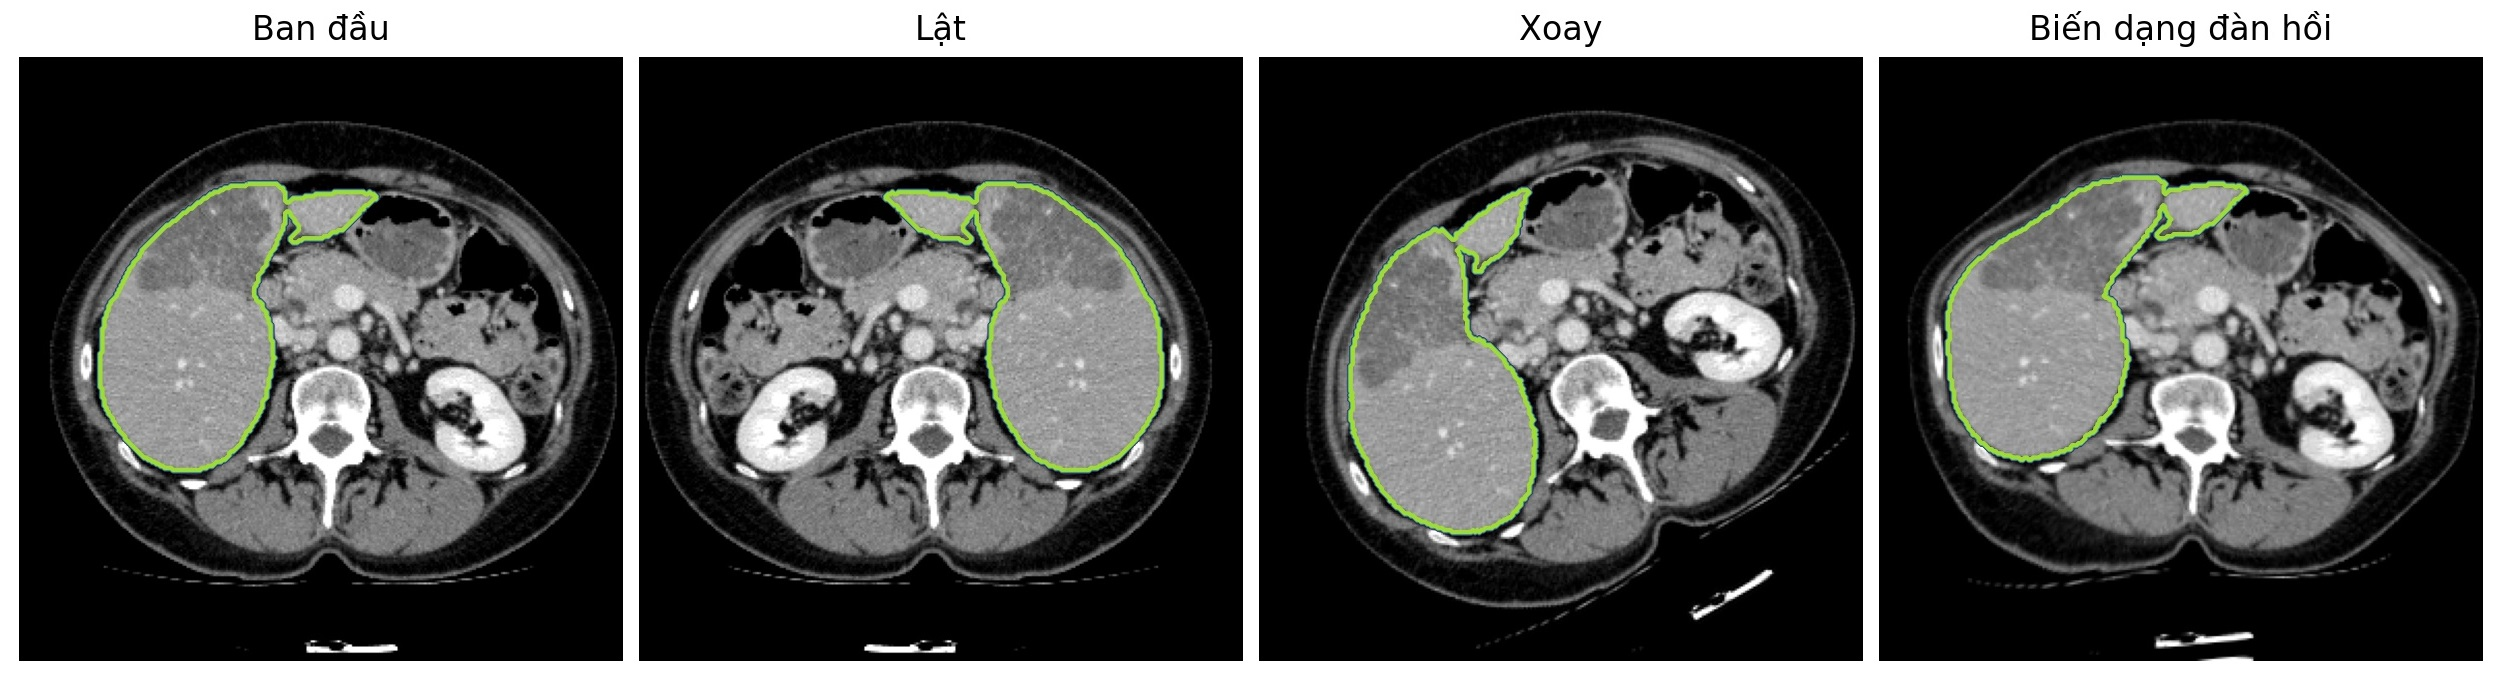
\includegraphics[width=14cm]{images/experience/aug.jpg}
    \caption{Ảnh trước và sau khi tăng cường dữ liệu}
\end{figure}
Thực tế khi chụp ảnh CT, bệnh nhân dược yêu cầu nằm ở một hướng cố định, kết quả là ảnh chụp cũng sẽ theo hướng cố định đó, việc lật và xoay ảnh sẽ không mang lại nhiều ý nghĩa trong thực tế. Tuy nhiên, việc có nhiều dữ liệu giúp mô hình học tập một cách tổng quát từ đó đem lại kết quả phân đoạn tốt hơn. Các phương pháp trên sẽ được nhóm sử dụng để tăng cường dữ liệu cho mô hình. \par

\subsubsection{Chia nhỏ dữ liệu}
Trong bài toán phân đoạn gan (mạch máu), dữ liệu ở dạng volume (mảng ba chiều) với kích thước lớn nhỏ khác nhau trong khi việc huấn luyện mô hình đòi hỏi dữ liệu đầu vào có cùng kích thước. Có nhiều cách để đưa dữ liệu về cùng kích thước như thêm đệm vào các volume kích thước nhỏ để đưa chúng về cùng kích thước với volume lớn nhất, thay đổi kích thước (resize) volume thành kích thước nhỏ hơn hoặc chia các volume thành nhiều sub-volume có kích thước giống nhau. Cách thứ nhất không khả thi vì giới hạn phần cứng, không thể huấn luyện mô hình với dữ liệu có kích thước lớn như vậy. Việc thay đổi kích thước volume như cách hai không bảo toàn khoảng cách không gian của các điểm dữ liệu, điều này làm mất đi ý nghĩa của việc nội suy để đưa các khoảng cách giữa ba chiều của các ảnh về cùng một giá trị như ở trên. Do đó, nhóm đã lựa chọn cách thứ ba là chia nhỏ volume ban đầu thành nhiều sub-volume có kích thước giống nhau.\par
Có nhiều cách để chia một volume thành nhiều sub-volume như chọn ngẫu nhiên, chia tuần tự,... Giả xử volume V ban đầu có kích thước D x H x W với D, H, W lần lượt là chiều sâu, chiều dài và chiều rộng của volume, sub-volume $S_{i}$ có kích thước là T x T x T.\par
\begin{itemize}
    \item \textbf{Chọn ngẫu nhiên}: chọn ngẫu nhiên một điểm nằm trong volume V có tọa độ $(x, y, z)$ làm điểm bắt đầu sau đó chọn sub-volume $S_{i} = V[x+T, y+T, z+T]$. Lặp lại quá trình này cho đến khi đủ số lượng sub-volume cần tạo. Phương pháp này có ưu điểm là kiểm soát được số lượng sub-volume được tạo ra nhưng cũng có nhược điểm là có thể một số vùng dữ liệu trong volume V bị bỏ sót. Điều này có thể được khắc phục bằng cách tăng số lượng mẫu cần lấy, khi đó xác suất để một vùng trong ảnh bị bỏ sót sẽ thấp xuống.
    \item \textbf{Chia tuần tự}: sử dụng một cửa sổ có kích thước bằng với kích thước sub-volume để trượt từ đầu cho đến cuối volume giống như cách lớp tích chập trích xuất đặc trưng. Volume V được chia nhỏ thành nhiều sub-volume $S_{i}$, các sub-volume này có thể chồng lấp lên nhau hoặc không. Đệm đã được thêm vào volume V để số lượng sub-volume tạo ra là số nguyên.
\end{itemize}
\begin{figure}[H]
    \centering
    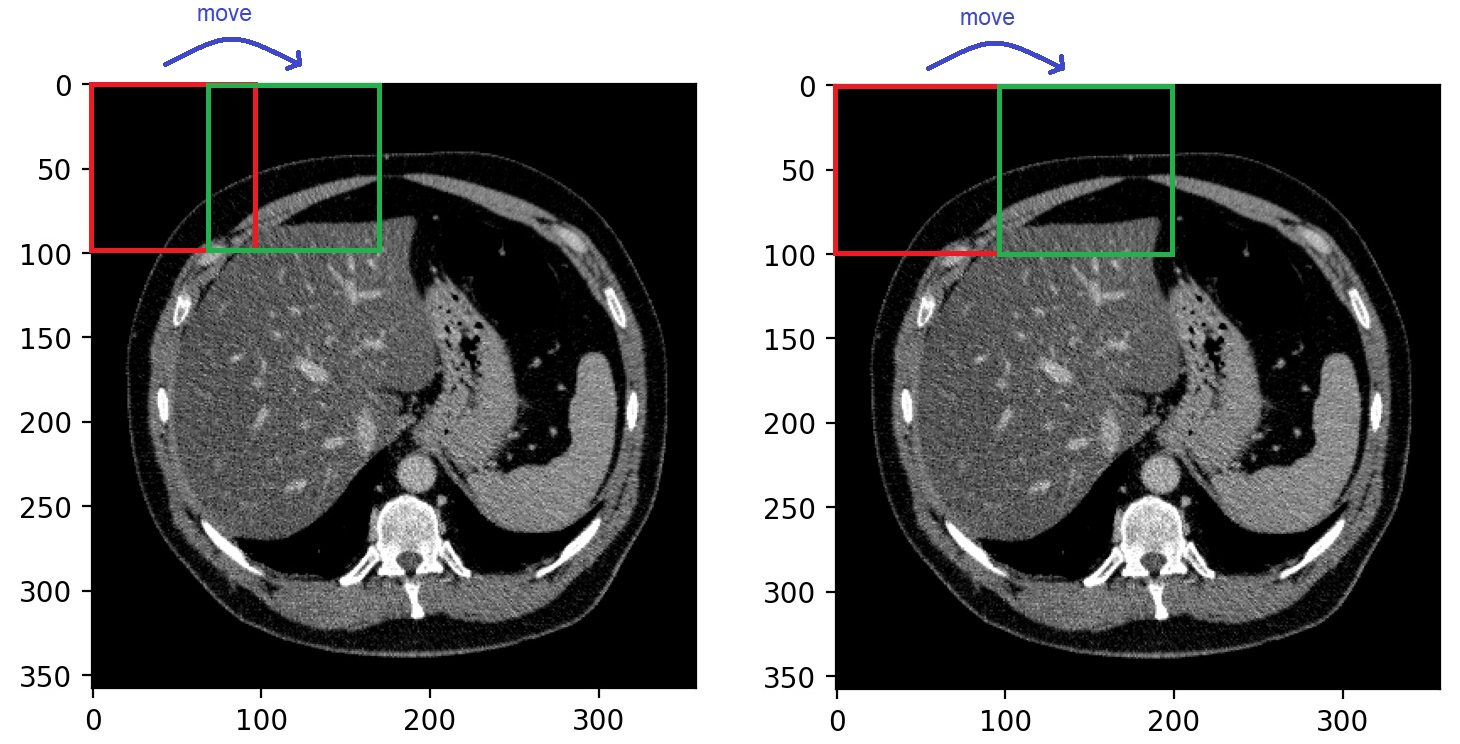
\includegraphics[width=12cm]{images/dataset/sub-volume-2d.jpg}
    \caption{Minh hoạ việc chia dữ liệu tuần tự}
    \label{2d_subvolume}
\end{figure} \par
Hình \ref{2d_subvolume} minh họa việc chia dữ liệu tuần tự trên một lát cắt (2D). Hình vuông màu đỏ là vị trí ban đầu của cửa sổ trượt, hình vuông màu xanh là vị trí tiếp theo. Ở hình bên trái, các sub-volume có chồng lấp lên nhau (phần giao nhau giữa hai hình vuông đỏ và xanh). Ở hình bên phải, các sub-volume nằm liên tiếp và không chồng lấp nhau. \par
Bước nhảy của cửa sổ trượt (stride) ảnh hưởng đến số lượng sub-volume được tạo ra. Nếu bước nhảy nhỏ hơn kích thước T, các sub-volume có chồng lấp lên nhau một phần, kết quả là tạo ra nhiều sub-volume hơn khi chia không chồng lấp. Nếu bước nhảy bằng T, các sub-volume sẽ nằm liên tiếp và không chồng lấp nhau. Nếu bước nhảy lớn hơn T, nhiều vùng dữ liệu sẽ bị bỏ sót, cách này sẽ không dược nhóm sử dụng trong các thí nghiệm sau này.

\subsubsection{Trích xuất thành phần gan}
Để tăng tính độ chính xác cho mô hình phân đoạn mạch máu, nhóm đã giới hạn lại phạm vi gắn nhãn cho mạch máu là chỉ quan tâm đến mạch máu nào thuộc vùng gan. Do đó đối với mô hình phân đoạn máu sẽ có sử dụng thêm một bước là trích xuất thành phần gan. Với điều này, chúng tôi đã giả định việc nhãn gan của ảnh CT là đã biết trước. Việc giả định nhãn gan có sẵn là khả thi trong thời điểm hiện tại, bởi hiên nay kết quả cao nhất trong lĩnh vực phân đoạn gan đã đạt trên 95\% d
độ chính xác. Do đó việc giả định này có thể chấp nhận được.

\begin{figure}[H]
    \centering
    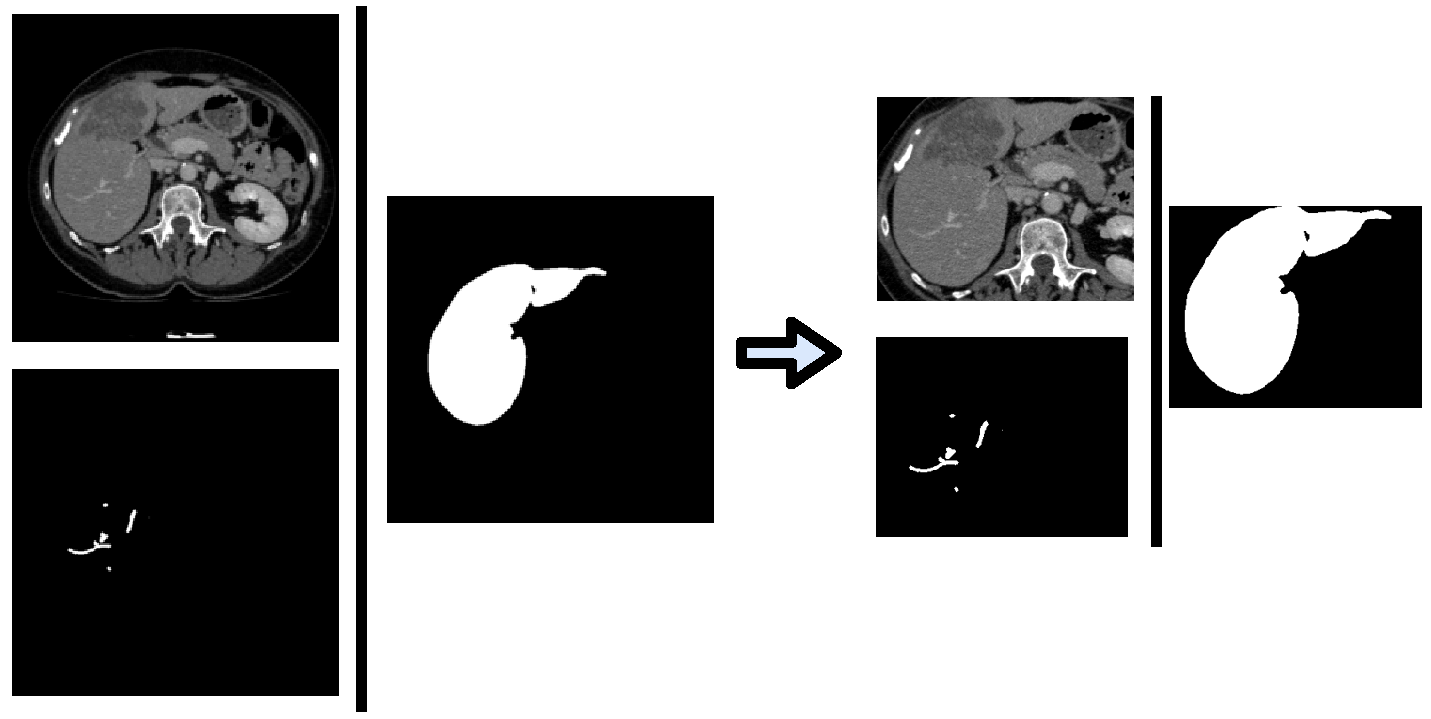
\includegraphics[width=12cm]{images/blood/extract_liver.pdf}
    \caption{Kết quả quá trình trích xuất thành phần gan.}
\end{figure}

\subsection{Trực quan hóa quy trình tiền xử lý}
\begin{enumerate}
    \item Lấy mẫu dữ liệu - đưa dữ liệu về kích thước chuẩn (1.0, 1.0, 1.0)mm đối với gan gà (0.5, 0.5, 0.5)mm đối với máu.
    \item Áp dụng ngưỡng dữ liệu [-100, 400].
    \item Chuẩn hóa HU về đoạn [0,1].
    \item Trích xuất thành phần gan.
    \item Chia tuần tự (hoặc ngẫu nhiên) thành các khối sub-volume nhỏ hơn.
\end{enumerate}
\begin{figure}[H]
    \centering
    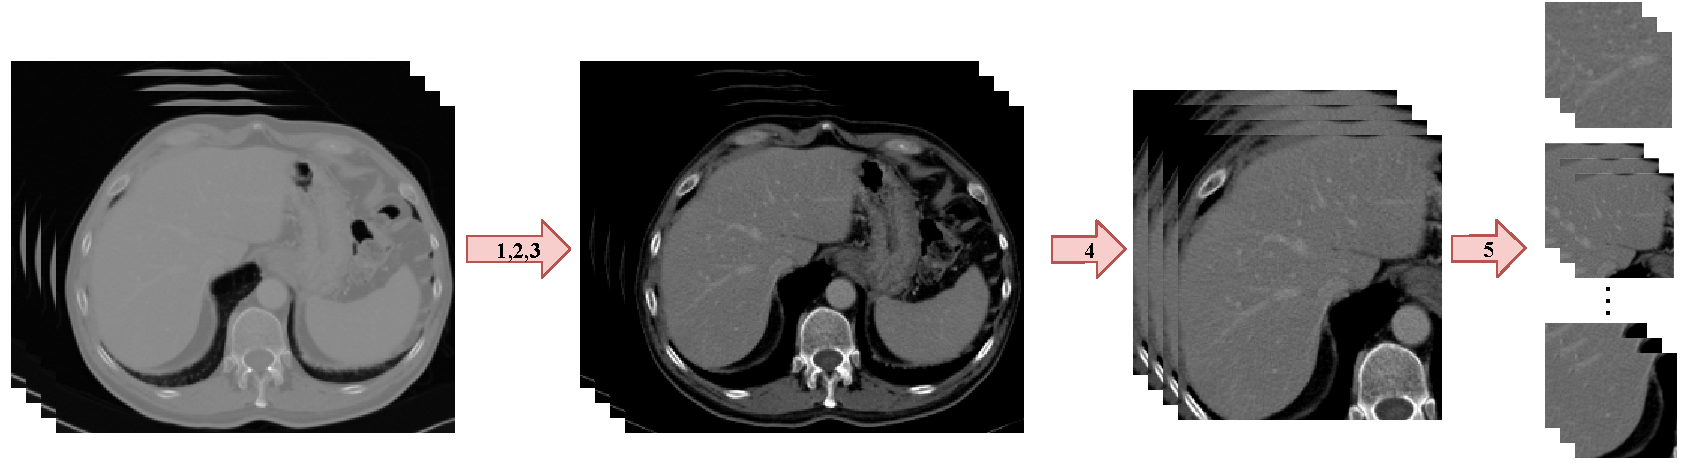
\includegraphics[width=14cm]{images/blood/preprocess_stage.pdf}
    \caption{Quy trình tiền xử lý.}
\end{figure}